\chapter{Forces à distance}
%
Une force modélise une action mécanique : un homme pousse un chariot, le chariot se met en mouvement. L'action est de pousser, c'est une action de contact, son effet est la mise en mouvement. Cette action peut être modélisée par une force : l'homme applique une force sur le chariot.

\begin{center}
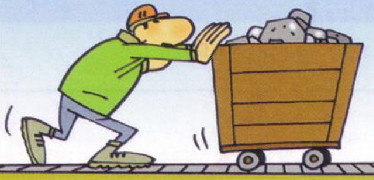
\includegraphics[scale=0.6]{./forces/chariotPousse}
\end{center}

Une force est représentée par un vecteur et un point d'application : Le point d'application est le point de contact (A), la force est horizontal, vers la droite et possède une valeur (mesurée en newton).

\begin{center}
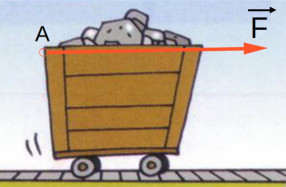
\includegraphics[scale=0.6]{./forces/chariotVecteur}
\end{center}

Nous étudions dans les paragraphes suivants, trois forces à distance (il n'y a pas de contact entre les corps).


%%%%%%%%%%%%%%%%%%%%%
\section{Force gravitationnelle}
%%%%%%%%%%%%%%%%%%%%%
%

L'interaction gravitationnelle est une action à distance entre les corps : les corps ayant une masse s'attirent entre eux, la force gravitationnelle modélise l'interaction gravitationnelle. 

La terre exerce sur la lune une action mécanique dont l'effet est d'{\it incurver} sa trajectoire, sans cette action la lune s'éloignerait de la terre.

\setlength{\unitlength}{1cm}
%
\begin{center}
\mbox{%\fbox{
\begin{picture}(17,3)
\put(2,2){\circle{1.52}}
\put(1.6,0.8){Terre}
\thicklines
\put(2,2){\vector(1,0){2.76}}
\put(4.3,2.3){$\overrightarrow{F}_{L/T}$}
\put(15,2){\circle{0.5}}
\put(14.6,1.2){Lune}
\thicklines
\put(15,2){\vector(-1,0){2.76}}
\put(12,2.3){$\overrightarrow{F}_{T/L}$}
\end{picture}}

$\overrightarrow{F_{L/T}}$ : Force gravitationnelle exercée par la lune sur la terre,

 $\overrightarrow{F_{T/L}}$ : Force gravitationnelle exercée par la terre sur la lune.
\end{center}


%%%%%%%%%%%%%%%%%%%%%%%%%%%%%%%%%%%%%%%%%%%%%%%%%%%%%%%%%%%%%%%%%%%%%%%%%%%%

%

%%%%%%%%%%%%%%%%%%%%%
\section{Champ électrique et potentiel scalaire}
%%%%%%%%%%%%%%%%%%%%%
%
Le champ électrique créé par une particule chargé s'étend dans l'espace à 3 dimensions. Il est possible, afin de simplifier les schéma de se limiter à 2 dimensions.

Le champ électrique créé par une particule chargée est radial et son amplitude décroit avec la distance à la particule.

\begin{center}
\tikzstyle{fleche}=[->,line width=1pt]
\begin{tikzpicture}
  \begin{scope}[xshift=0 cm,yshift=0 cm, scale = 1.6]%
\foreach \t in {60,120, ...,360}
\draw [fleche] (\t:1) -- (\t:2.8);
\foreach \t in {30,90, ...,360}
\draw [fleche] (\t:2) -- (\t:2.45);
\foreach \t in {15,45,-15,-45}
\draw [fleche] (\t:3) -- (\t:3.2);
\foreach \t in {15,45,-15,-45}
\draw [fleche] (\t+180:3) -- (\t+180:3.2);
\draw [fill=red] (0,0) circle(0.1) node [above right] {$Q_1$};
  \end{scope}
\end{tikzpicture}
\end{center}


Comme le champ de pente dérive d'un champ scalaire (le champ d'altitude), le champs electrique dérive d'un champ scalaire. On l'appelle le potentiel électrique. On représente ci-dessous les lignes de même potentiel (équi-potentiel) du potentiel électrique créé par une particule chargée.

\begin{center}
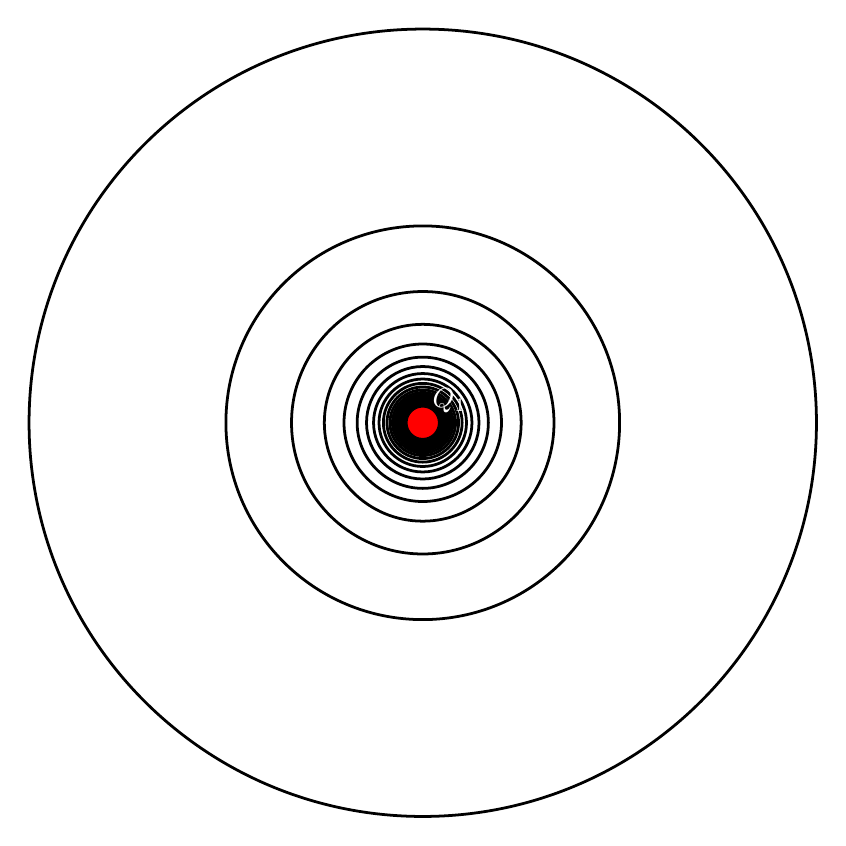
\begin{tikzpicture}
  \begin{scope}[xshift=0 cm,yshift=0 cm, scale = 1]%
\foreach \t in {1,2, ...,30}
\draw [line width=1pt] (0,0) circle (5/\t) ;

\draw [fill=red] (0,0) circle(0.2) node [above right,text=white] {$Q_1$};
  \end{scope}
\end{tikzpicture}
\end{center}

En 3 dimensions, les points de même potentiel sont des surfaces. Les surfaces équi-potentiel du potentiel créé par une particule chargée sont des sphères.

%%%%%%%%%%%%%%%%%%%%%%%%%%%%%%%%%%%%%%%%%%%%%%%%%%%%%%%%%%%%%%%%%%%%%%%%%%%%

%

%%%%%%%%%%%%%%%%%%%%%
\section{Force magnétique}
%%%%%%%%%%%%%%%%%%%%%
%

La force magnétique est la force qui s'exerce entre les \textbf{\textit {aimants}}.
Les aimants sont des matériaux possédant des propriétés magnétiques.
Certain métaux peuvent être aimantés par la proximité d'un aimant.

\subsection{Pôles magnétiques}

Un aimants est toujours {\it orienté}, il possède un pôle dit \textbf{\textit {nord}} et un pôle
dit \textbf{\textit {sud}}.


\subsection{Action magnétique}

La force magnétique entre deux aimants, est attractive et répulsive, elle exerce un {\it couple} :
entre deux aimants, les pôles opposés s'attirent, les pôles identiques se repoussent. 

Ci-dessous, deux aimants sont schématisés, les pôles nord en rouge et les pôles sud en bleu. On ne représente que les forces que l'aimant 2 exerce sur l'aimant 1.

\begin{center}
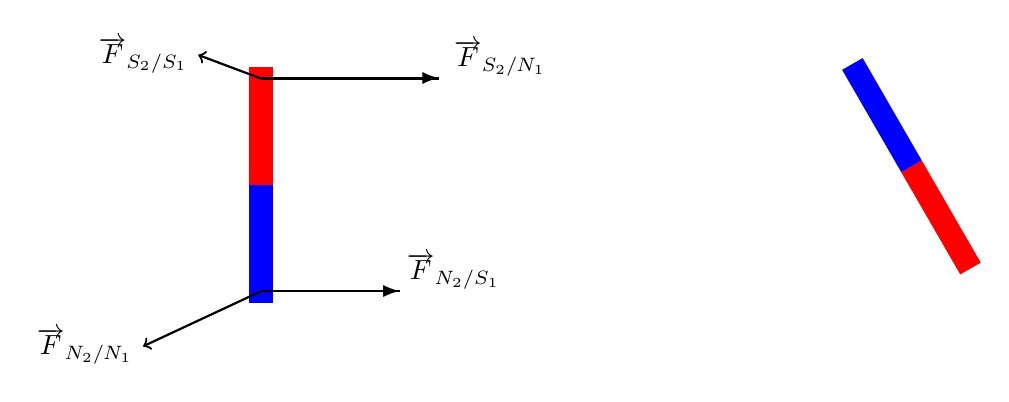
\begin{tikzpicture}[scale=1]
\fill [blue] (0,0) rectangle (0.3,1.5);
\fill [red] (0,1.5) rectangle (0.3,3);
\begin{scope}[rotate=30,yshift=-4.2cm]%
\fill [red] (8,0) rectangle (8.3,1.5);
\fill [blue] (8,1.5) rectangle (8.3,3);
\end{scope}
\thicklines
\put(0.15,0.15){\vector(1,0){1.76}}
\put(2,0.3){$\overrightarrow{F}_{N_2/S_1}$}

\put(0.15,2.85){\vector(1,0){2.26}}
\put(2.6,3){$\overrightarrow{F}_{S_2/N_1}$}

\draw [thick] [->] ((0.15,(0.15) --++(-1.5,-0.7) node [left] {$\overrightarrow{F}_{N_2/N_1}$};

\draw [thick] [->] ((0.15,(2.85) --++(-0.8,0.3) node [left] {$\overrightarrow{F}_{S_2/S_1}$};

%\put(0.15,0.15){\vector(-1,-1){0.5}}
%\put(4.3,2.3){$\overrightarrow{F}_{L/T}$}
\end{tikzpicture}
\end{center}
%%%%%%%%%%%%%%%%%%%%%%%%%%%%%%%%%%%%%%%%%%%%%%%%%%%%%%%%%%%%%%%%%%%%%%%%%%%%

%
%\input{.//.tex}
